\documentclass[10pt,conference]{IEEEtran}
% \IEEEoverridecommandlockouts
% The preceding line is only needed to identify funding in the first footnote. If that is unneeded, please comment it out.
\usepackage{cite}
\usepackage{amsmath,amssymb,amsfonts}
\usepackage{algorithmic}
\usepackage{graphicx}
\usepackage{textcomp}
\usepackage{xcolor}

\usepackage{listings}
\usepackage{xcolor}


% tables
\usepackage{multirow}

\newcommand\question[1]{{\color{violet}#1}}
\newcommand\todo[1]{{\color{red}#1}}


\definecolor{codegreen}{rgb}{0,0.6,0}
\definecolor{codegray}{rgb}{0.5,0.5,0.5}
\definecolor{codepurple}{rgb}{0.58,0,0.82}
\definecolor{backcolour}{rgb}{0.97,0.97,0.97}

\lstdefinestyle{mystyle}{
    backgroundcolor=\color{backcolour},
    commentstyle=\color{codegreen},
    keywordstyle=\color{magenta},
    numberstyle=\tiny\color{codegray},
    stringstyle=\color{codepurple},
    basicstyle=\ttfamily\footnotesize,
    breakatwhitespace=false,
    breaklines=true,
    captionpos=b,
    keepspaces=true,
    numbers=left,
    numbersep=5pt,
    showspaces=false,
    showstringspaces=false,
    showtabs=false,
    tabsize=2
}

\lstset{
%   basicstyle=\ttfamily,
  mathescape
}



\usepackage{minted}
\usepackage{hyperref}

% to manually equalize the lengths of two columns on the last page
%  of your paper;
\usepackage{balance}

\usepackage{caption} 
\captionsetup[table]{skip=10pt}

% for affilation
\usepackage{authblk}

% \bibliographystyle{ieeetr}

\def\BibTeX{{\rm B\kern-.05em{\sc i\kern-.025em b}\kern-.08em
    T\kern-.1667em\lower.7ex\hbox{E}\kern-.125emX}}
\begin{document}

\title{Distilled Sparse Linear Algebra in Hardware 
}

% \author{\IEEEauthorblockN{Aleksey Tyurin}
% alekseytyurinspb@gmail.com
% \and
% \IEEEauthorblockN{Ekaterina Vinnik}
% catherine.vinnik@gmail.com
% \and
% \IEEEauthorblockN{Daniil Berezun}

% d.berezun@2009.spbu.ru
% \and
% \IEEEauthorblockN{Semyon Grigorev}
% s.v.grigoriev@spbu.ru
% \andIEE
% }

\author[1,3]{Aleksey Tyurin}
\author[1,3]{Ekaterina Vinnik}
\author[1,2,3]{Daniil Berezun}
\author[1,2,3]{Semyon Grigorev}

\affil[1]{\footnotesize Saint Petersburg State University, Saint Petersburg, Russia}
\affil[2]{\footnotesize JetBrains Research, Saint Petersburg, Russia}
\affil[3]{\footnotesize alekseytyurinspb@gmail.com, catherine.vinnik@gmail.com, d.berezun@2009.spbu.ru, s.v.grigoriev@spbu.ru}


\maketitle

%% Abstract
%% Note: \begin{abstract}...\end{abstract} environment must come
%% before \maketitle command
\begin{abstract}

  Sparse linear algebra is widely used in graph processing, machine learning, and computational biology. 
  And whilst in dense applications fusion optimization is extensively used to reduce the number of kernel calls and memory accesses it is hard to support in case of sparse applications due to the considerably irregular nature of the latter.
  Fusion is also a well-studied optimization in the world of functional programming where it is often needed to remove intermediate data structures to achieve near imperative languages performance.
  We propose the usage of functional compressed representation for sparse data and a functional language to express sparse linear algebra algorithms to be able to utilize distillation: the technique which provides fusion and partial evaluation, enhances asymptotic time and guarantees a specific structure of the output programs.
  Next, we suggest using hardware code generation to convert our optimized programs into highly parallel and pipelined hardware to increase performance. 
  The work presents some intermediate evaluation of this approach.
  % Sparse linear algebra is a great framework for building algorithms in a uniform and optimization-amenable way.
% However, CPUs and GPUs currently running such algorithms are underutilized due to being too general-purposed for problems that include sparsity.
% Thus, an application-specific integrated circuit could speed sparse computations up, following the example of \textit{Google TPU's}.
% It is worth noting that such a circuit needs to be not self-contained to allow some expected optimizations to be made by a compiler or a framework itself.
% Finally, the optimizations should be easily definable in the language and as automated as possible, thus a careful simultaneous design of hardware and software is needed.
% The proposal describes the bottlenecks inherent to present sparse linear algebra framework implementations, summarizes the expected optimizations, and proposes a co-design approach to designing a highly-optimized sparse linear algebra framework.
% \textit{This is a work in progress and not yet present the final result}.


\end{abstract}


\section*{Introduction}


Linear algebra is a great instrument for solving a wide variety of problems utilizing matrices and vectors for data representation and analysis with the help of highly optimized routines.
But in reality matrices in many applications are often sparse, incurring both computational and storage inefficiencies, requiring unnecessarily large storage, occupied by zero elements, and a large number of operations on zeroes, where the result is obviously known beforehand. 
The traditional approach to address these inefficiencies is to compress the matrix and store only the non-zero elements and then operate only on the non-zero values.
It makes the techniques of matrix compressed representation and sparse linear algebra to be an effective way of tackling problems in areas including but not limited to graph analysis~\cite{GAILLA}, computational biology~\cite{compBio} and machine learning~\cite{Kepner_2017}.

% And whilst the matrices involved in a vast diversity of modern applications, e.g., recommender~\cite{gupta2020architectural,amazon} systems and graph analysis~\cite{graph1,graph2}, consist of a large number of elements, the major part of them are zeros.

% Such a high sparsity incurs 
% Thus, the effect of matrices tending to be sparse in many applications makes the techniques of matrix compressed representation and sparse linear algebra to be the effective way of tackling problems in areas including but not limited to graph analysis~\cite{GAILLA}, computational biology~\cite{compBio} and machine learning~\cite{Kepner_2017}.

\emph{GraphBLAS}~\cite{buluc2017graphblas} standard defines sparse linear algebra building blocks useful to express algorithms for already mentioned areas in a uniform way in terms of sparse matrix and vector operations over some semiring.
These include, for instance, matrix/vector multiplication, element-wise operations (e-wise for short), Kronecker product, masking, i.e. taking a subset of elements that satisfies the mask or its complement, etc., and are sufficient to express a lot of algorithms, e.g. \emph{PageRank}, \emph{Breadth-First-Search}, \emph{Sparse Deep Neural Network}~\cite{SparseDNN}.

% Sparse linear algebra defines building blocks for expressing algorithms for already mentioned areas in a uniform way in terms of sparse matrix and vector operations over some semiring. 
% Once such blocks are implemented in software (or hardware) a myriad of expressible algorithms could be tuned and optimized at once by optimizing and tuning the building blocks.
% \emph{GraphBLAS}~\cite{buluc2017graphblas} standard summarizes such blocks, including but not limited to matrix/vector multiplication, element-wise operations (e-wise for short), kronecker product, masking, i.e. taking a subset of elements that satisfies the mask or its complement. These are sufficient to express a lot of algorithms, e.g. \emph{PageRank}, \emph{Breadth-First-Search}, \emph{Sparse Deep Neural Network}~\cite{SparseDNN}. The parameterizability by a semiring is the key to expressivity since the behaviour of each operation is fully customized.
% \emph{GraphBLAS}~\cite{buluc2017graphblas} standard,
% There are several implementations of GraphBLAS standard showing decent performance for both GPU~\cite{yang2020graphblast} and CPU~\cite{SuiteSparse} backends with one of them already speeding up graph database queries~\cite{redis}.
% The standard itself is a C API specification that standardizes sparse linear algebra building blocks initially for graph computations, but nevertheless applicable in other areas. 
% It translates mathematical specification to API that could be efficiently implemented in hardware or software. 
% Also it is the only such specification and has been completed by researchers from the field of high-performance graph algorithms based on sparse linear algebra. 
% The specification further gives the means for interoperation with vertex-centric libraries, which potentially makes it a crucial component in the future ecosystem of big graphs~\cite{sakr2020future}.
% A list of operations provided by the standard constitutes (the list is not exhaustive) matrix/vector multiplication, element-wise operations (e-wise for short), kronecker product, masking, i.e. taking a subset of elements that satisfies the mask or its complement. These are sufficient to express a lot of algorithms, e.g. \emph{PageRank}, \emph{Breadth-First-Search}, \emph{Sparse Deep Neural Network}~\cite{SparseDNN}. Notably each operation is parameterizable by a semiring, which is the key to expressivity since the behaviour of each operation is fully customized.

However sparse computations appear to have a low arithmetic-to-memory operations intensity, meaning that the main bottleneck of sparse algorithms is the sparse representation itself that induces pointer-chasing and presents irregularity of memory accesses.
Thus, a number of optimizations have been identified~\cite{yang2020graphblast}, whose aim is to reduce the intensity of memory accesses and the one considered in this work is \emph{fusion}. \emph{Fusion} simply stands for gluing several functions into one to remove intermediate data structures, namely those that are first constructed and then deconstructed.
There are two types of fusion that we are interested in.

\begin{figure}
  \centering
  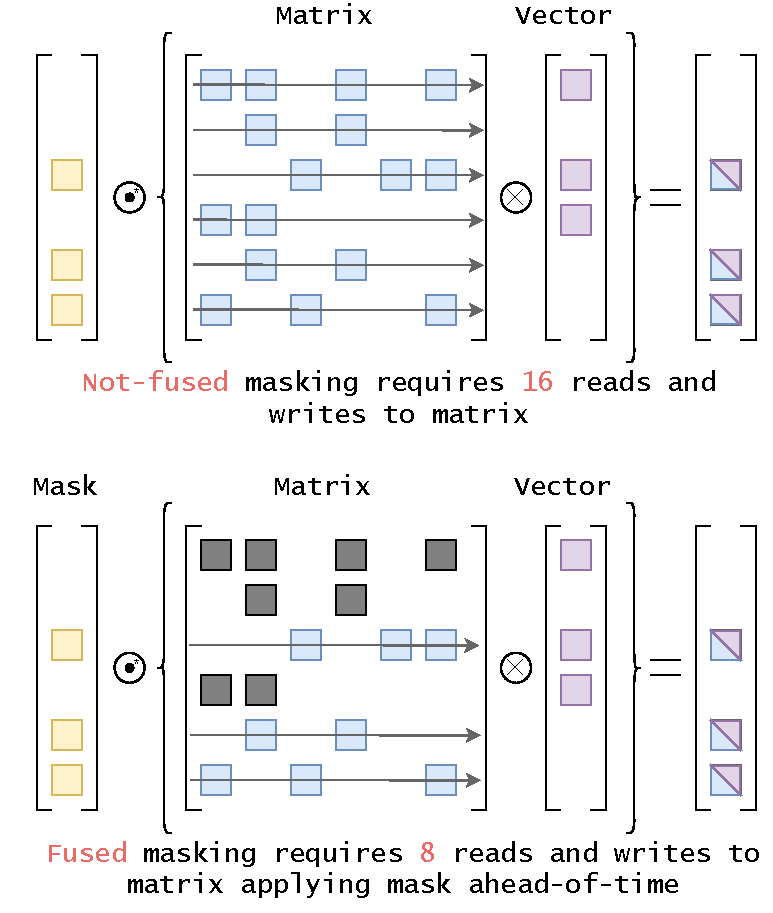
\includegraphics[width=\linewidth]{figs/MaskFusionIA3_2.pdf}
  \caption{Mask fusion}
  \label{fig:mask_fusion}
\end{figure}

\begin{figure*}[t]
  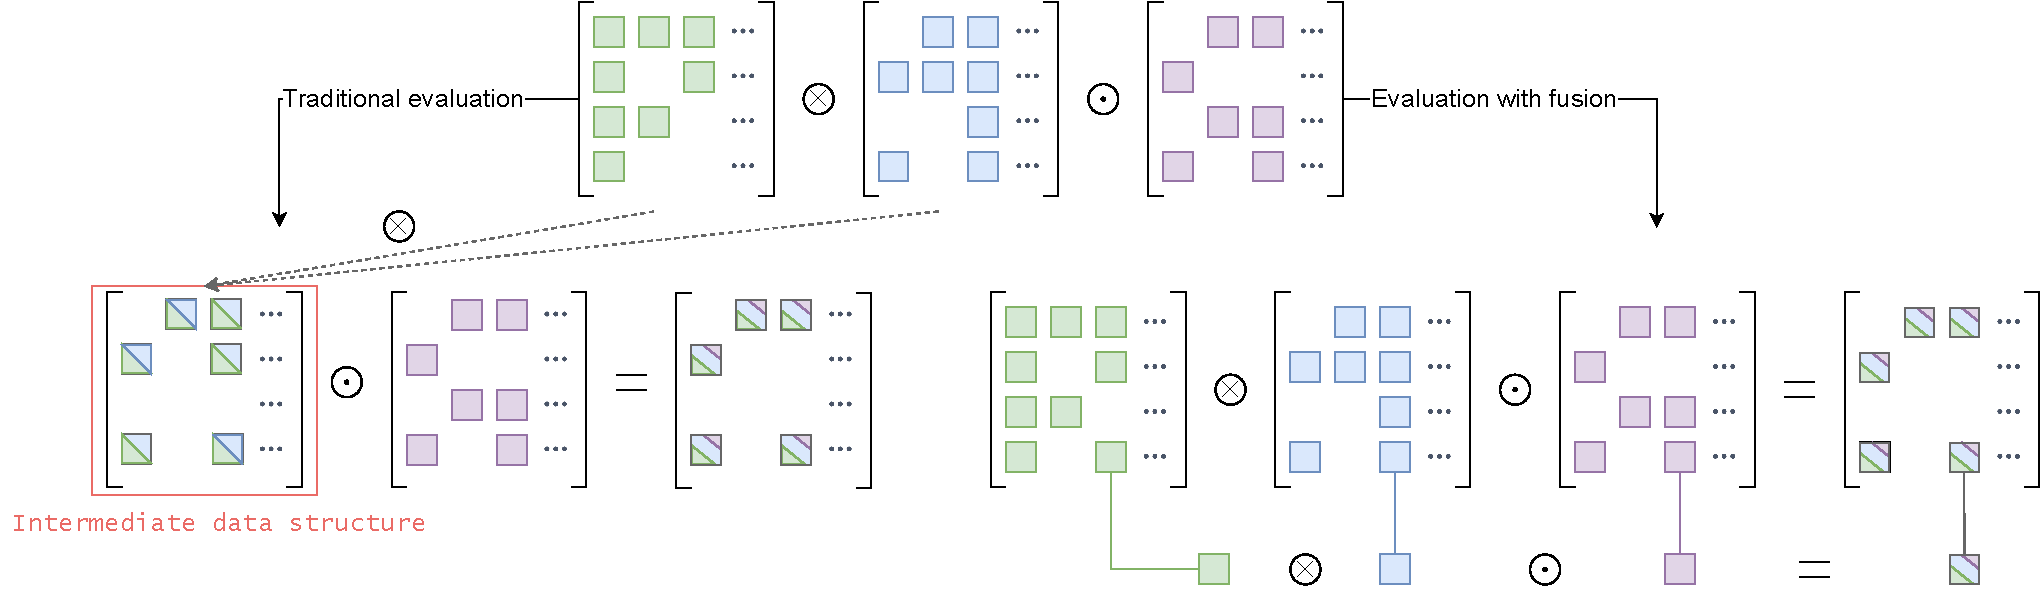
\includegraphics[width=\textwidth]{figs/KernelFusionIA3_2.pdf}
  \caption{Kernel fusion}
  \label{fig:kernel_fusion}
\end{figure*}

\paragraph*{Mask fusion}
Ahead-of-time masking could reduce the number of memory accesses in case of, e.g., matrix-vector multiplication by taking only the elements of interest.
In order to achieve such a behavior, a mask should be fused (i.e. transformed into a single operation) with the corresponding operation, for the operation to perform computations only for the elements in the mask.
The effect of masking in the case of sparse matrix-dense vector multiplication could be seen in figure~\ref{fig:mask_fusion}.
Ahead-of-time masking reduces the number of memory accesses from 16 to 8.


\paragraph*{Kernel fusion}
it is responsible for fusing arbitrary operations to explicitly remove intermediate data structures as could be seen from figure~\ref{fig:kernel_fusion}.
In a traditional way of evaluation having consecutive operations leads to the creation of intermediate data structures, which first should be constructed and then deconstructed to create another data structure, fusion is in charge of removing them.


In the case of loop-based programming fusion simply stands for joining several loops into one to increase memory locality and reduce the number of required iterations.
It is a crucial technique in dense applications and is usually followed by a stage of \emph{polyhedral analysis}.
This is extensively exploited in frameworks like TensorFlow and its XLA compiler~\cite{TensorFlowXLA}, where fusion is used to merge several GPU kernels into one to reduce both memory transfer and kernel start overheads. 

Some general-purpose solutions exist that support fusion, e.g., \cite{Futhark} which are based on map/reduce semantics.
But in order to support sparse operations, they should be able to fuse across index arithmetic, which is not the case.
Also at the moment neither ~\cite{SuiteSparse}  nor ~\cite{yang2020graphblast} have adopted the fusion in their implementations.
In this work, we propose an approach to support fusion for such applications and outline the overall solution design as well as present some intermediate evaluations of the approach.

\section{Solution}

The problem of intermediate data structures is natural for functional programming and
a number of approaches for fusion have been designed, namely \emph{partial evaluation, deforestation, supercompilation, distillation} \cite{jones, WADLER1990231, supercompilation, distillation}.
In this work, we will focus on \emph{distillation} since it is capable of the same as other approaches but is able to produce a superlinear improvement for the program being optimized~\cite{distillation} and imposes a specific structure of the output programs, namely tail modulo cons where each function call is at most tail-recursive wrapped with a constructor application.

For successful fusion the compressed representation should be fuseable, i.e., it should avoid indexing and be natural to the functional paradigm.
A quad-tree representation~\cite{qtree} looks promising in this case. 
The implementation of this compressed representation as an algebraic data type is straightforward and could be seen in listing~\ref{lst:qtree}, it recursively splits a matrix into four submatrices.

\begin{listing}

  \begin{minted}[]{Haskell}

  data QTree a = QNone  
               | QVal a 
               | QNode (QTree a) (QTree a)
                       (QTree a) (QTree a) 
  
  \end{minted}
  \caption{Quad-tree compressed representation}
  \label{lst:qtree}
  
  \end{listing}


\begin{figure*}[t]
  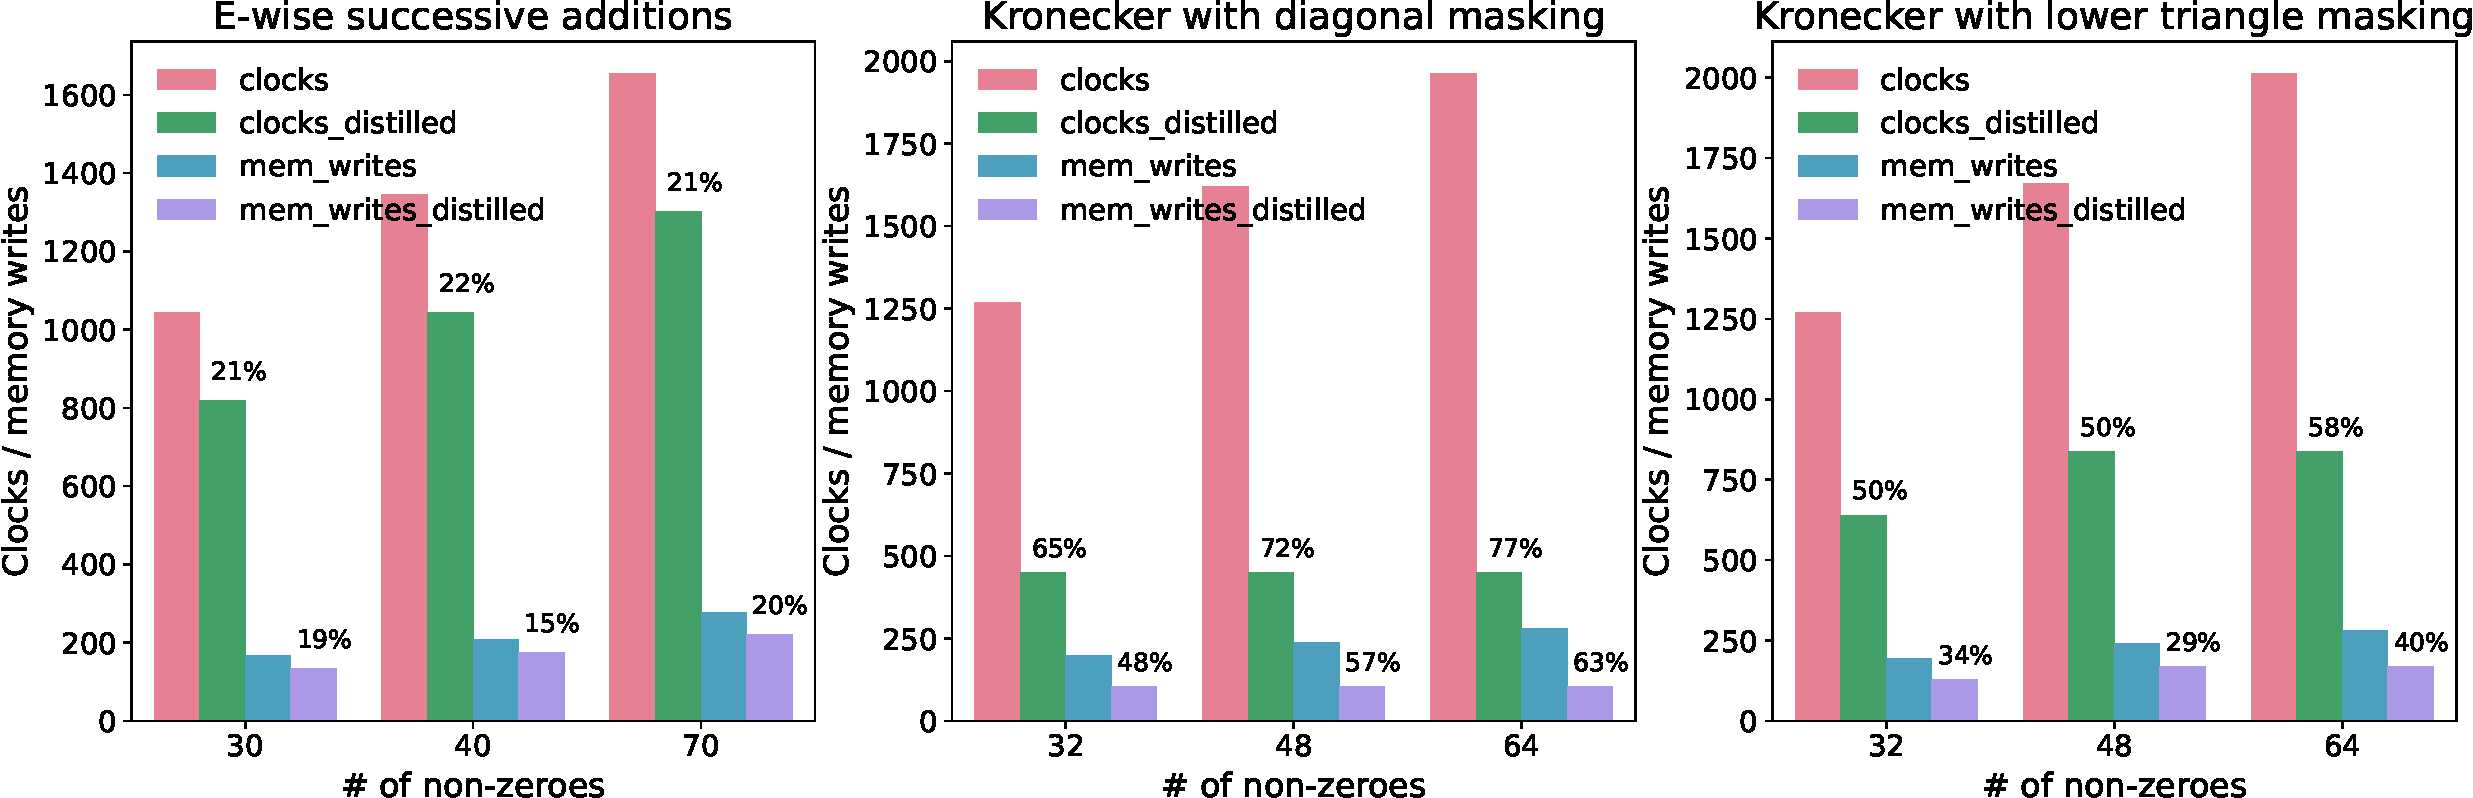
\includegraphics[width=\textwidth]{figs/HardwareBenchs_3.pdf}
  \caption{Hardware evaluation}
  \label{fig:evaluation}
\end{figure*}



\begin{table*}[t!]
  \centering
  \begin{tabular}{ |c|c|c|c|c|c|c|c|} 
\hline
\multirow{2}{5em}{Function} & \multirow{2}{5em}{Matrix size} & \multicolumn{2}{c}{Reductions} \vline & \multicolumn{2}{c}{Memory reads} \vline& \multicolumn{2}{c}{Ratio}\vline\\
\cline{3-8}
{}&{}&Original&Distilled&Original&Distilled&Reductions&Memory reads\\
\hline
E-wise additions & 64 & 20317 & 11459 & 3170 & 2372 &56\% &74\%\\
E-wise additions & 2048 & 139851 & 81907 & 20351 & 15056 & 58\% & 73\%\\
Kronecker with triangle masking & 64 & 535125 & 367868 & 92470 & 67110 & 68\% & 72\%\\
Kronecker with triangle masking & 2048 & 1215051 & 827020 & 212133 & 151601 & 68\% & 71\%\\
\hline

\end{tabular}
  \caption{Software evaluation}
  \label{tab:table_distill}
\end{table*}

What is more important is that sparse linear algebra routines based on this representation are in a divide-and-conquer form and thus are parallelizable. 
To increase the performance of function programs we aim to generate an FPGA-kernels from them and at the moment we use FHW project~\cite{funcHLS} for this, which generates parallel and pipelined dataflow hardware from arbitrary Haskell programs.
This approach is also aimed to bridge the gap between our solution and existing sparse linear algebra frameworks: widely used compressed representations could be first converted into quad-tree representation and then our kernels could be called from existing frameworks written in C/C++.

\section{Distillation}
Distillation~\cite{distillation} is the evolution of the deforestation approach, which was designed to eliminate intermediate trees and lists in functional programs making them as performant as their imperative counterparts.
Distillation is a transformation algorithm, which is able to produce superlinear improvement in the runtime of programs. 
Basically, it glues a sequence of several possibly recursive functions into one possibly recursive function.
It is doing so by symbolically applying normal order reduction rules to all possible branches of a program, which is called \emph{driving}, generating a process tree where each node is an expression.
The topmost node represents the sequence of functions we want to fuse, and when a similar node is encountered at the bottom of the tree the driving is stoped and a residual program is generated from the tree where such similar nodes represent a new recursive function call, the result of fusion.

Also, the algorithm imposes a tail modulo cons structure on the output program, which 
eases the translation into hardware and mitigates the requirements for garbage collection, which is not implemented yet in the hardware compiler that we use~\cite{funcHLS}. 
Both these properties are useful but are not used at the moment.


\section{FHW project}

FHW~\cite{funcHLS} is a Haskell-to-System-Verilog compiler that supports functions with arbitrary recursion, which is a problem for most modern high-level synthesis tools.
It encodes algebraic data types in hardware and provides a distinct memory space for each.
It also provides some optimizations for divide-and-conquer programs which is just the case for our compressed representation of choice.
The exact implementation of memory for each type is fully customizable, so the memory for quad-trees could be implemented in any way, e.g. supporting multiple parallel reads/writes for subtrees.


\section{Evaluation}

The distillation is supported for a toy functional language shipped with the distiller, so we implement a set of sparse linear algebra routines in this language leaving everything which is not expressible in the language as free variables, e.g., integers and primitive operations for them.
Then the program in this language is distilled and translated into Haskell. Then free variables are substituted with corresponding values and the program is translated into System Verilog using FHW.
We use Vivado to simulate generated programs and count the number of clock cycles and memory writes performed during the simulation. 
The result of evaluation could be seen in figure~\ref{fig:evaluation} where we compare distilled and non-distilled programs that were translated into hardware.

The leftmost example is the distillation of a sequence of element-wise additions, which appear for example in Luby’s maximal independent set algorithm and is the case of kernel fusion. 
It could be seen that the fused program is up to 20\% more efficient in terms of both clock cycles and memory writes. 
The number of non-zeroes is the sum of the number of non-zeroes for each matrix (there are three 8x8 matrices). The number of non-zeroes is small due to the fact that the compiler does not support external memory at the moment, thus the construction of matrices should be part of the program itself and the simulator is not comfortable with huge input programs. Also, it is easier to manually count the number of memory writes when the order of matrices is small.

The other two examples are masked Kronecker products, i.e. the case of mask fusion. Here the number of non-zeroes is the number of non-zeroes in the result of Kronecker product before masking, which is also a 8x8 matrix.
Since the mask fusion allows to perform evaluation only for the needed elements, fusion provided up to 77\% improvement in clock cycles and up to 63\% in memory writes for diagonal mask and up to 58\% fewer clock cycles and 40\% less memory writes for lower triangle masking. 

We also evaluated the enhancement brought by fusion using the interpreter of the toy language using the corresponding interpreter and boolean matrices with the structure from~\cite{SuiteSparseMatrixCollection}. The results of this evaluation could be seen in the table~\ref{tab:table_distill}.
Reductions are the number of reductions rules applied during interpretation while memory reads is the number of \texttt{case e} contexts encountered where expression \texttt{e} is deconstructed. The improvement is up to 70\% in terms of both reductions and memory reads. 

The exact transformation performed by the distiller could be seen in listing~\ref{lst:fusion_listing}, which is a simplified excerpt from Luby’s maximal independent set algorithm. The series of e-wise additions create an intermediate \texttt{new\_members} matrix which is eliminated after fusion where all three matrices are destructed in one top-level case expression.

The evaluation shows that sparse linear algebra routines are suitable for fusion with distillation giving noticeable performance both in software and hardware. The hardware part is prominent since it allows to join fusion and sparse hardware where memory could be implemented in the most effective way, unlike modern CPUs and GPUs which perform poorly in sparse applications. The software and hardware benchmarks are available at~\cite{YaccPOT} and~\cite{FHWME} respectively.

\begin{listing}

  \begin{minted}[fontsize=\footnotesize]{Haskell}

eWiseAdd g m1 m2 =
  case m1 of{
    QNone -> m2;
    QVal v1 -> case m2 of
          QNone -> m1;
          QVal v -> QNode (g v1 v);
          QNode t1 t2 t3 t4 -> error
    QNode q1 q2 q3 q4 -> case m2 of 
          QNone -> m1
          QVal v -> error
          QNode t1 t2 t3 t4 -> QNode
                                (eWiseAdd g q1 t1)
                                (eWiseAdd g q2 t2)
                                (eWiseAdd g q3 t3)
                                (eWiseAdd g q4 t4)}

main = ...
        let new_members = eWiseAdd gt prob neighbor_max 
            iset' = eWiseAdd lor iset new_members in
        ...
--gets fused into
main = ...

    let iset' = case iset of
                ... -> case neighbor_max of
                    ... -> case prob of ...
-- @new_members has been eliminated
  \end{minted}
  \caption{Fusion by means of distillation}
  \label{lst:fusion_listing}
  
\end{listing}

\section{Conclusion}

In this work, we proposed the approach of supporting fusion for sparse linear algebra applications using distillation and functional programming.
To achieve better performance of functional programs we translate them into System Verilog using a hardware compiler. We presented the evaluation of the approach both in software and hardware which showed prominent results.
Future work includes the improvement of the hardware compiler. We want to evaluate divide-and-conquer hardware optimizations as well as to design an efficient memory for quad-tree compressed representation.
Also, we want to support external memory to be able to evaluate large real-world examples. Finally, the overall solution could be shipped as a library of OpenCL-like FPGA kernels to be able to utilize it in current workflows.


%% Bibliography
\bibliographystyle{./IEEEtran}
\bibliography{bib}


%% Appendix
% \appendix
% \section{Appendix}

% Text of appendix \ldots


\end{document}